
\documentclass[tikz,convert={outfile=\jobname.svg}]{standalone}
\usepackage{pgfplots}
\usetikzlibrary{calc,patterns,snakes}
% \usetikzlibrary{...}% tikz package already loaded by 'tikz' option
\begin{document}
    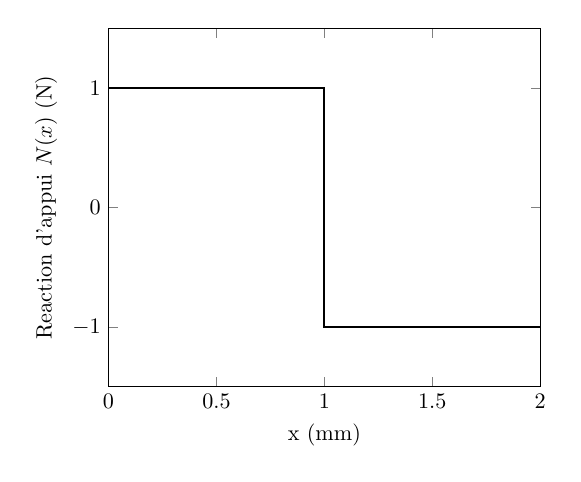
\begin{tikzpicture}[scale=0.8]
      \begin{axis}[xlabel=x (mm), ylabel=Reaction d'appui $N(x)$ (N), xmin=0,ymin=-1.5,xmax=2,ymax=1.5]
	\addplot [thick,color=black, mark=none] coordinates {(0,1) (1,1) (1,-1) (2,-1)};
      \end{axis}
    \end{tikzpicture}
\end{document}